\section{Image Processing Deep Neural Networks}\label{sec:image-processing-deep-neural-networks}

%Checked
\subsection{Overview of Convolutional Neural Networks}\label{subsec:convolutional-neural-networks}

Convolutional neural networks (CNNs) constitute a class of deep learning models that are commonly used for computer vision tasks
including image classification, object detection, and segmentation.
Given the ability of convolutional neural networks (CNNs) to learn spatial hierarchies of features and their various types of data representations
(bounding box, segmentation mask, etc.), they are made ideal for the task of traffic object detection.
Many recent advances  in computer vision have been made possible by CNNs, including the development of models such as YOLO, Faster R-CNN, and ResNet.
A dozen of these models have been developed, each with its own unique architecture and capabilities.
However, they all share the same fundamental principles gathered recently by Jiuxiang Gu in his 2018 work,
\("\)Recent advances in convolutional neural networks\("\)~\cite{GU2018354}.

The designation of the class is derived from the utilisation of convolutional layers, which apply filters to the input
data in order to extract features, outside convolutional layers, CNNs also comprise pooling layers, fully
connected layers.

These models are employed in a multitude of applications, including autonomous vehicles, surveillance systems, and medical imaging.
As these applications align with the project's objectives, these types of neural networks are selected for the task of traffic object detection.

The subsequent paragraphs will provide an overview of the essential components of convolutional neural networks (CNNs).

\paragraph{Convolutional layers}\label{par:convolutional-layers}

Convolutional layers  represent the fundamental building blocks of convolutional neural networks (CNNs).
Convolution operations are applied to the input data using filters (or in other word kernels) that process the input image.
This process enables the model to identify local patterns such as  edges, textures, and shapes.
Each convolutional layer generates a set of feature maps,
which indicate the presence of different types of these aforementioned features in the input.
These feature maps are then passed to the subsequent layers for further processing, such as pooling or classification,
to refine the information coded into the image.
During the training phase, the parameters of the kernels are learned (their values are adjusted),trough backpropagation,
allowing the network to enhance feature extraction for specific tasks.


\begin{figure}[h]
\centering
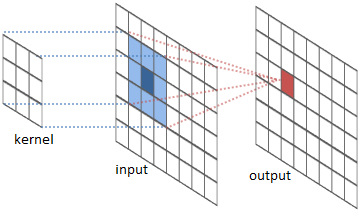
\includegraphics[width=.50\textwidth]{figures/convolution}
\caption{Convolutional layer operation~\cite{article}}
\label{fig:convolution}
\end{figure}

\paragraph{Sampling layers}\label{par:sampling-layers}

The objective of sampling layers is to reduce the dimensionality of the data set while ensuring the preservation of the
input data's essential features.
Sampling can entail the application of techniques such as subsampling or strided convolutions,
whereby a specific stride is applied to the convolution operation in order to down-sample the feature maps.

\paragraph{Pooling layers}\label{par:pooling-layers}

The objective of pooling layers is to reduce the spatial dimensions of feature maps given by the convolutional layers,
thereby decreasing the number of parameters and computations in the network.
Moreover, this process enhances the model's resilience to minor
translations in the input data by mitigating the effects of potential outliers.
The most prevalent forms of pooling are max pooling and average pooling.
Max pooling selects the maximum value from a specified window, whereas average pooling computes the average.
By down-sampling the feature maps, pooling layers assist in maintaining the most important features while discarding less
critical information from the picture, also efficient in reducing the computational load.



\begin{figure}[h]
\centering
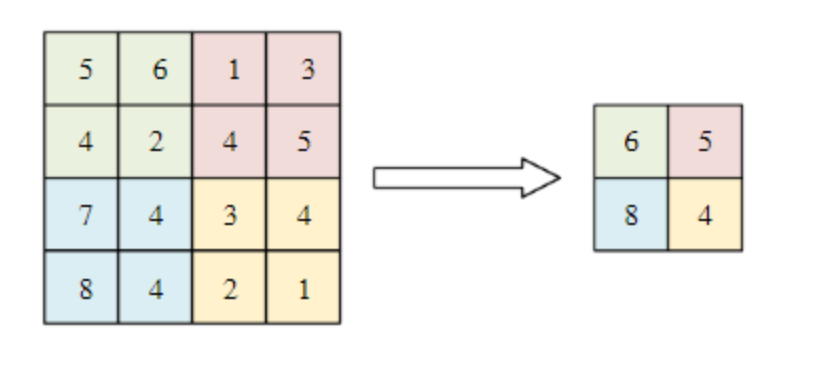
\includegraphics[width=.50\textwidth]{figures/pooling}
\caption{Pooling layer operation~\cite{article}}
\label{fig:pooling}
\end{figure}

\paragraph{Fully connected layers}\label{par:fully-connected-layers}

Fully connected layers, also referred to as dense layers, are typically located at
the conclusion(HEAD) of convolutional neural network (CNN) architectures.
In these layers, each neuron is connected to every neuron in the preceding layer.
This structure enables the model to integrate information from all features and make final predictions.
Fully connected layers are particularly useful in classification tasks,
where they compute the output probabilities for each class based on the features extracted by the preceding layers.
Regularisation techniques, such as dropout, are frequently employed in these layers to prevent overfitting.
\begin{figure}[ht]
\centering
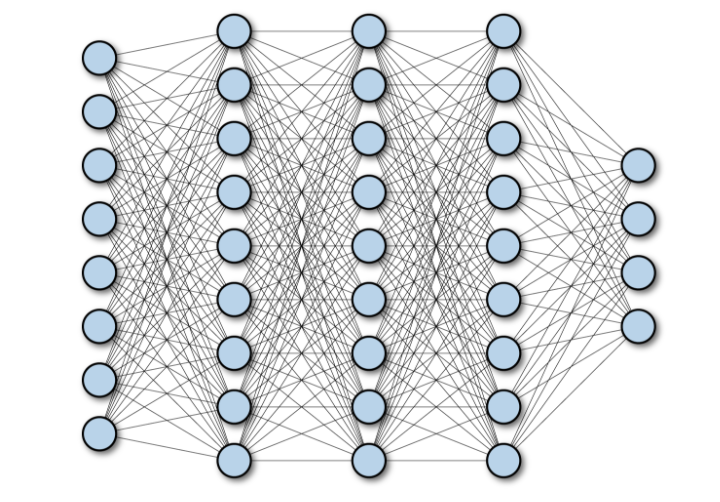
\includegraphics[width=0.50\textwidth]{figures/fully connected}
\caption{Fully Connected Layer semantics~\cite{article}}
\label{fig:fullconn}
\end{figure}

\subsection{Activation Functions}\label{subsec:activation-functions}

Activation Functions are utilised in CNNs(and other Neural networks) to introduce non-linearity into the model.
They assist the model in learning complex patterns and making accurate predictions.
 In light of the work conducted by Siddharth Sharma and Simone Sharma regarding  activation functions~\cite{sharma2017activation}
the most prevalent  activation functions are ReLU, Sigmoid, and Tanh.
Although alternative activation functions, such as BSF and ELU, could be employed, they are not utilised by the examined model (Yolov8).
Consequently, a detailed discussion of these functions will not be provided.
The following paragraphs  will discuss the ReLU, Sigmoid, and Tanh activation functions based on the work of Siddharth and Simone Sharma\cite{sharma2017activation}.


\begin{figure}[h!]
    \centering


    \begin{subfigure}[b]{0.5\textwidth}
        \centering
        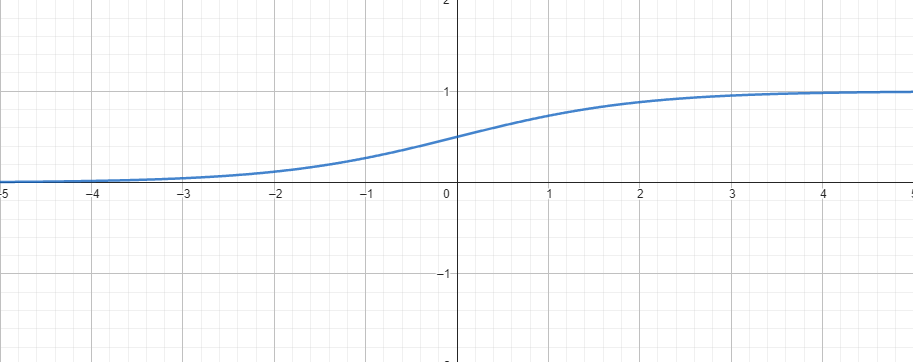
\includegraphics[width=\textwidth]{figures/sigmoid}
        \caption{Sigmoid activation function}
        \label{fig:sigmoid}
    \end{subfigure}
    \hfill
    \begin{subfigure}[b]{0.45\textwidth}
        \centering
        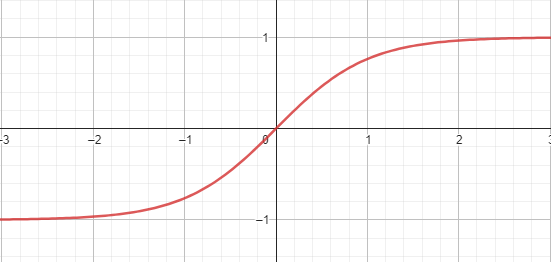
\includegraphics[width=\textwidth]{figures/tanh}
        \caption{Tanh activation function}
        \label{fig:tanh}
    \end{subfigure}
    \hfill
    \begin{subfigure}[b]{0.45\textwidth}
        \centering
        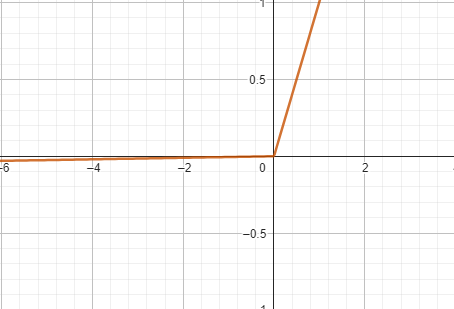
\includegraphics[width=\textwidth]{figures/relu}
        \caption{ReLU activation function}
        \label{fig:relu}
    \end{subfigure}

    \caption{Activation functions: Sigmoid,Tanh and ReLU}
    \label{fig:activation_functions}
\end{figure}


\paragraph{ReLU}\label{par:relu}
The Rectified Linear Unit (ReLU) is one of the most common and easy to understand activation functions in convolutional neural networks (CNNs).
It is defined as \( f(x) = \max(0, x) \) in the works of Siddharth Sharma~\cite{sharma2017activation}.
This function introduces non-linearity while maintaining a simple and efficient computation.
The ReLU function helps mitigate the vanishing gradient issue, allowing models to learn faster and perform better.
However, be susceptible to the phenomenon known as the \("\)dying ReLU\("\) problem, where neurons become inactive and only output zeros,
particularly during the training of deep networks.



\paragraph{Sigmoid}\label{par:sigmoid}
The Sigmoid function translates input values to a range between 0 and 1,
rendering it useful for binary classification problems.
It is defined as \( f(x) = \frac{1}{1 + e^{-x}} \) in the works of Siddharth Sharma~\cite{sharma2017activation}.
While the Sigmoid function provides smooth gradients,
it is prone to the vanishing gradient problem,
especially for large positive or negative input values.
This can slow down the training of deep networks,
which is why it is often replaced by other activation
functions in hidden layers,
though it still finds use in the output layer for binary classification tasks.



\paragraph{Tanh}\label{par:tanh}
The hyperbolic tangent (Tanh) function is another activation function that maps input values to a range between -1 and 1.
It is defined as  \( f(x) = \frac{e^x - e^{-x}}{e^x + e^{-x}} \)in the works of Siddharth Sharma~\cite{sharma2017activation}.
The Tanh function is zero-centered and centricaly symmetrical, facilitates the centring of the data and may result in accelerated convergence during training.
Nevertheless, it continues to exhibit the vanishing gradient problem for large input values, though to a lesser extent than the Sigmoid function.



\subsection{Introduction to YOLO}\label{subsec:introduction-to-yolo}

The YOLO (You Only Look Once) model is a relatively recent object detection system that is straightforward to utilise and comprehend, while also benefiting from a thriving community of users and developers.
It is based on the YOLO algorithm , which is a real-time object detection algorithm developed by Joseph Redmon and Ali Farhadi in 2015\cite{redmon2016lookonceunifiedrealtime}.

Unlike traditional object detection methods that apply classifiers to various sections of an image,
YOLO approaches the problem as a single regression problem.
The algorithm divides the image into a grid and  predicts bounding boxes and class probabilities parallel for each grid cell,
thereby enabling the detection of multiple types and instances of objects in a single run.
This architecture not only enhances speed but also improves detection accuracy by reducing the number of false positives.

The YOLO model has evolved through multiple versions, with improvements in both performance and varying capability.
Subsequent versions of the model, including YOLOv2, YOLOv3, and the latest YOLOv5 and YOLOv7, as well as Yolov8 (with Yolov10 and 11 forthcoming),
have introduced advancements in network architecture,
feature extraction, and training techniques.
These developments have rendered YOLO a suitable candidate for a plethora of applications,
including autonomous vehicles, as evidenced by the author's own observations, surveillance systems, and real-time video analysis.

A further noteworthy attribute of the Yolo-type neural networks is their scalability and versatility in terms of model architecture.
These models are available in a range of sizes (\textit{nano, small, medium, large, extralarge}) and with a variety of detection types (\textit{semantic segmentation, bounding boxes,
oriented bounding boxes, instance segmentation}), which can be deployed in diverse scenarios.




\begin{figure}[ht]
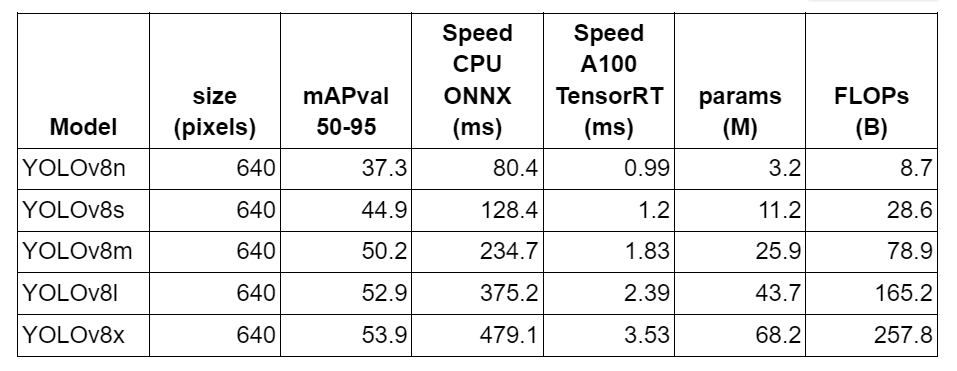
\includegraphics[width=1.0\textwidth]{figures/table1}
\caption{Different sizes of the YOLOv8~\cite{githubGitHubUltralyticsultralytics}}
\label{fig:tableofsizes}
\end{figure}

%táblázat a Yolo architektúrákról és méreteikről hasznos lehet ide

\subsection{Model architecture}\label{subsec:architecture}
This network, like many others in the CNN family, has a distinctive architectural configuration that
enables the execution of intricate tasks such as object detection and classification.
The system is constituted of three distinct and discrete components,
each comprising a unique set of layers that perform specific and separate functions.

\begin{figure}[ht]
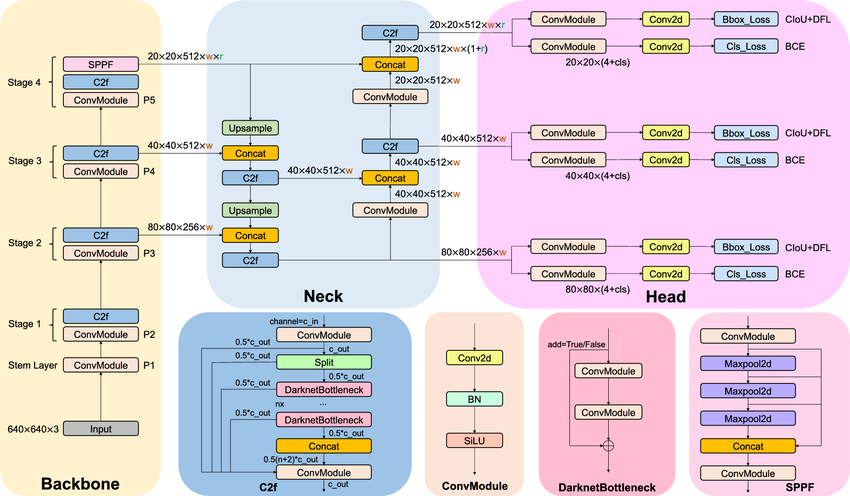
\includegraphics[width=1.0\textwidth]{figures/Detailed-illustration-of-YOLOv8-model-architecture-The-Backbone-Neck-and-Head-are-the}
\caption{The architecture of the YOLOv8 model~\cite{FractureDetection2024}}
\label{fig:architecture}
\end{figure}

\paragraph{Backbone}\label{par:backbone}
The YOLOv8 model is based on convolutional neural networks (CNNs) that have been specifically designed to capture essential features from input images.
It comprises multiple layers of convolutional operations (called Conv and a complex layer called C2F)
that extract progressively more sophisticated representations.
This structure emphasises both depth and computational efficiency,
enabling the model to discern subtle details while maintaining rapid processing capabilities.
Innovations such as skip connections and normalization techniques are employed to enhance the learning dynamics and improve the model's robustness to variations in input conditions.
%kép a backbone-ról

\paragraph{Neck}\label{par:neck}
In the YOLOv8 architectural design, the neck serves as an intermediary between the backbone and the head.
The primary function of the neck is to consolidate features from the various levels of the backbone,
thereby enhancing the model's ability to detect objects across different scales.
By employing strategies such as feature fusion or pyramid pooling,
the neck effectively integrates both coarse and fine features,
enabling the model to better handle overlapping objects and diverse scene contexts.
This feature aggregation is crucial for optimising the detection performance,
as it allows the model to harness a comprehensive range of information.

%kép a neckről


\paragraph{Head}\label{par:head}
The head of the YOLOv8 model is responsible for generating the final outputs,
which are based on the features that have been processed through the neck.
The final stage of the YOLOv8 model translates the aggregated feature maps into bounding box predictions and associated class scores for each detected object.
This section typically employs a combination of convolutional and fully connected layers to refine these outputs,
ensuring they are accurate and meaningful.
Additionally, the head may implement techniques such as adaptive anchors or
confidence scoring to enhance the localisation and classification accuracy.
By effectively synthesising the rich feature information, the head enables YOLOv8 to achieve high-performance object detection suitable for a wide array of applications.

%kép a headről
\subsection{Training}\label{subsec:training}
The training process~\cite{redmon2016lookonceunifiedrealtime} for the YOLOv8 model involves feeding its input with a large dataset of labeled images.
The model learns to identify objects by minimizing the difference between its predictions and the actual labels trough multiple iterations:
After a training cycle ,if the default settings are kept, a validation function (so called val) is run,
to determine more information on the model's performance on pictures that are not present in the training set.
The training process is iterative, with the model adjusting its parameters to improve its predictions over time.
This process is computationally intensive and requires access to powerful hardware,
the best fitting hardware for this purpose, that can be found in an ordinary PC, is the GPU\@.

The training process involves several key steps, including data preprocessing, model initialization,
loss calculation, and parameter optimization.
The model is trained using a technique called backpropagation,which involves adjusting the model's weights based on
the error between its predictions and the ground truth labels.

The Yolov8 model uses a number of different loss functions,according to the original paper~\cite{redmon2016lookonceunifiedrealtime}
, loss functions to measure the difference between its predictions and the actual labels in different ways:



\begin{itemize}
\item \textbf{CIoU (Complete Intersection over Union) loss}:
\[
\text{CIoU} = 1 - \left( \text{IoU} - \frac{\rho^2(\mathbf{b}, \mathbf{b}^g)}{c^2} - \alpha v \right) ~\cite{li2020generalizedfocallosslearning}
\]
where \(\rho\) is the Euclidean distance between the center points of the predicted box \(\mathbf{b}\) and
 the ground truth box \(\mathbf{b}^g\), \(c\) is the diagonal length of the smallest enclosing box covering
 the two boxes, \(\alpha\) is a positive trade-off parameter, and \(v\) measures the consistency of aspect
 ratio.
 It is more sensible to localisation accuracy.

\item \textbf{DFL (Distribution Focal Loss)}:
\[
\text{DFL} = -\sum_{i=1}^{N} p_i \log(q_i)~\cite{DBLP:journals/corr/abs-1911-08287}
\]
where \(p_i\) is the true probability distribution and \(q_i\) is the predicted probability distribution.
It is sensible to the accuracy classification.
\item \textbf{BCE (
binary cross-entropy for classification loss
)}:
\[
\text{BCE} = -\sum_{i=1}^{N} y_i \log(p_i) + (1 - y_i) \log(1 - p_i)~\cite{ruby2020binary}
\]
where \(y_i\) is the true label and \(p_i\) is the predicted probability.

\end{itemize}



I opted for training the model on my local machine, using a single GPU, while it provided me with sufficient performance
, the training time was significantly longer than it would have been on a more powerful cloud machine.
To reduce the chance of overfitting, the training dataset is typically divided into training and validation sets,
with the latter used to evaluate the model's performance on unseen data.
The trainings batch size where set to 3, which is not common, but it was necessary to fit the model on the GPU,
to optimise training time.

\subsection{Training and evaluation with the help of MLOps solutions}\label{subsec:training-and-evaluation-with-the-help-of-mlops-solutions}
In order to monitor the performance of the model and to facilitate the visualisation of the learning process,
as well as to organise the experiments, an online machine learning monitoring solution, Comet.ml, has been selected.
This tool is capable of tracking the training process in real time and of visualising the properties of the model on
a user-friendly dashboard, which can be accessed from any device with an internet connection.
The Comet.ml platform also provides a range of features that can be used to compare different experiments,
such as hyperparameter tuning, model versioning, and collaboration tools, while also offering a comprehensive
set of APIs for integration with other tools and platforms.

\begin{figure}[ht]
\centering
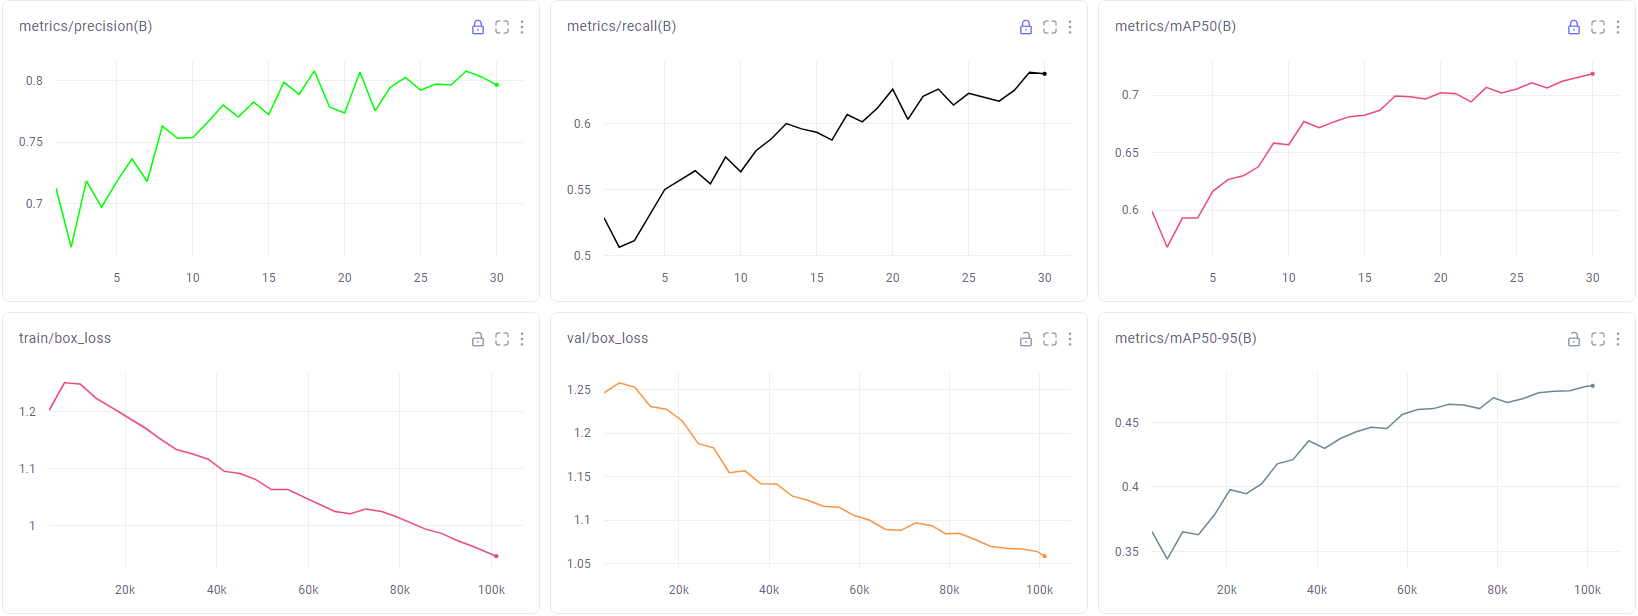
\includegraphics[width=1.0\textwidth]{figures/model}
\caption{Comet.ml dashboard about our the moodel}
\label{fig:comet}
\end{figure}

Figure~\ref{fig:comet} depicts the Comet.ml dashboard, which offers a comprehensive representation of the training process,
encompassing loss and accuracy metrics, the learning rate, and the model's performance on the validation set.
This information is vital for evaluating the model's performance and for identifying potential issues that may arise during training.
Furthermore, the Comet.ml platform enables the comparison of different experiments,
which can be beneficial for fine-tuning the model's hyperparameters and for improving its performance.
Which I did try out, for comparing the performances of the same model on the same dataset,
but with different epochs and batch sizes to see and find a good balance between training time and performance.